\section{Security}
Security generically refers to the \textbf{possibility} of \textbf{‘protecting’ information}, which is either stored in a \textbf{computer system} or transmitted on a \textbf{network}, against different types of attacks. The reason why security is so important is because there are now many computer systems that share resources (\textit{system security}) and a wide spread of distributed systems (\textit{network security}): notice that in this course we'll deal with both types of security.

The main areas involved in this process of security are telecommunications, electrical power systems, gas and oil etc.., while some examples of threats (or attacks) that may jeopardize their security are:

\begin{itemize}
    \item \textit{DoS};
    \item \textit{Modified DBs};
    \item \textit{Virus};
    \item \textit{Identity theft};
    \item ...
\end{itemize}

\subsection{Security properties}
There are many different aspects we might want to protect. We list the most important ones below. Each of them correspond to a different security property:

\begin{itemize}
    \item \textbf{Authenticity}: an \textbf{entity} should be \textbf{correctly identified}. This may apply to different settings. For example, the \textit{login} process allows for authenticating a user, a \textit{digital signature} (that we will discuss) allows for authenticating the entity originating a message, and so on;
    \item \textbf{Confidentiality} (or secrecy): \textbf{information} should only be \textbf{accessed} (read) by \textbf{authorized entities}. \textit{Confidentiality} involves, in turn, two aspects:

    \begin{itemize}
        \item \textit{Data confidentiality}, i.e. confidential \textbf{information} is \textbf{not disclosed} to unauthorized individuals;
        \item \textit{Privacy}, i.e. individuals \textbf{control} what information related to them may be collected and stored and by whom and to whom that information may be disclosed.
    \end{itemize}

    In general, in order to ensure confidentiality we need to use the \textit{"need to know"} basis for data access:

    \begin{itemize}
        \item How do we know \textit{who needs what} data? A possible approach would be to implement an access control that specifies \textit{who} can access \textit{what}, similarly to the UNIX permissions;
        \item How do we know a user \textit{is the person she claims to be}? In this case we need her identity and we need to verify this identity, and a possible approach would be of implementing an identification and authentication.
    \end{itemize}

    Notice that \textbf{confidentiality} is both \textbf{difficult} to \textbf{ensure}, and it is the \textbf{easiest} to \textbf{assess} in terms of success, since it is \textbf{binary} in nature (either we ensure confidentiality or not);
    
    \item \textbf{Integrity}: \textbf{information} should only be \textbf{modified} by \textbf{authorized entities}. Again, there exist two types of integrity:

    \begin{itemize}
        \item \textit{Data integrity}, which ensures that \textbf{information} and \textbf{programs} are \textbf{changed} only in a \textbf{specified and authorized manner};
        \item \textit{System integrity}, which ensures that a \textbf{system} performs its \textbf{intended function}, free from unauthorized manipulation.
    \end{itemize}

    Notice that there is a \textbf{difference} between integrity and confidentiality, in the sense that integrity is concerned with unauthorized \textit{modification} (i.e. \textit{write}) of the resources (assets), while confidentiality only deals with the \textit{access} (i.e. \textit{read}) to the assets. In this sense, \textbf{integrity} is \textbf{more difficult to measure} than confidentiality, also because of the fact that it is \textbf{not binary}, i.e. we can have different degrees of integrity. Finally, integrity is \textbf{context-dependent}, meaning that it refers different things in different contexts. 

    \underline{Example}: if we consider a quote from a politician, we can either preserve the quote (in this case we consider \textit{data integrity}, i.e. we preserve the content of the quote), or preserve the mis-attribute (in this case we consider the \textit{origin integrity}, i.e. we preserve the origin of the quote, the name of the politician).

    \item \textbf{Availability}: \textbf{information} should be \textbf{available}/\textbf{usable} by \textbf{authorized} users. This property is important to guarantee \textbf{reliability} and \textbf{safety}, since apart from attacks, availability might be lost in case of faults. This is addressed through techniques that make the system \textbf{fault-tolerant} and that we will not treat in this course. In general, we can say that an asset is available if:

    \begin{itemize}
        \item Timely request response, i.e. whenever we ask the asset, the system provides it;
        \item Fair allocation of resources, i.e. no starvation occurs;
        \item Fault tolerant, i.e. no total breakdown occurs;
        \item Easy to use in the intended way;
        \item Provides controlled concurrency (concurrency control, deadlock control etc..).
    \end{itemize}
    
    \item \textbf{Non-repudiation}: an \textbf{entity} should \textbf{not be able} to \textbf{deny} an \textbf{event}, for example, having sent/received a message. This property is crucial for e-commerce, where ‘contracts’ should not be denied by the parties;
    
\end{itemize}

There are, of course, many more properties that we do not mention here and we will not have time to address in this course. Examples are:

\begin{itemize}
    \item Fairness of contract signing;
    \item Privacy;
    \item Anonymity;
    \item Unlinkability, i.e. an attacker cannot distinguish if two items are related or not;
    \item Accountability, i.e. tracing an event to a unique entity. Notice that there's a difference between authenticity and accountability, since the former refers to the property of being able to be verified and trusted, while the latter refers to the possibility of tracing back an action to an entity.
\end{itemize}

\subsection{Typical attacks}
We assume information is flowing from a source to a destination. For example, reading data is a flow for the data container (e.g. a file) to a user while writing (or modifying) is a flow from a user to the file system, an so on.

\begin{figure}[h!]
    \centering
    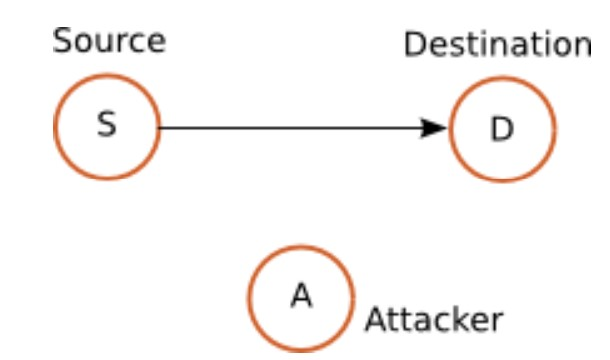
\includegraphics[scale = 0.7]{img/sec1.jpg}
    \label{sec1}
    \caption{Expected information flow}
\end{figure}

\textbf{Malicious users} might try to subvert the above properties in many different ways. We now give very general classification depending on how an attacker might interfere on the expected flow of information.

\subsubsection{Interruption}
In this case the \textbf{attacker stops the flow of information}. This is typically a \textbf{DoS} that makes the system/network unusable:

\begin{figure}[h!]
    \centering
    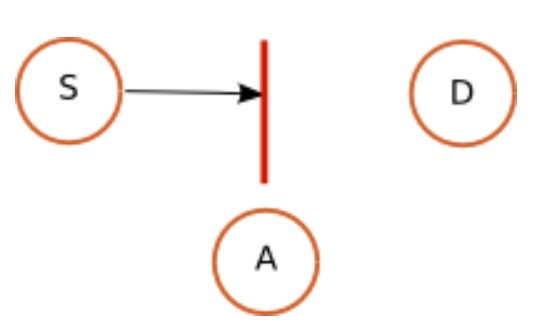
\includegraphics[scale = 0.7]{img/sec5.jpg}
    \label{sec5}
    \caption{The attacker interrupts the flow of information}
\end{figure}

An interruption breaks system \textbf{integrity} and \textbf{availability}, both because the message is not arriving to the destination. In general, an interruption is quite easy to notice, and some examples are DoS, canceling programs or data files, destruction of part of the hardware etc..

\subsubsection{Eavesdropping (or interception)}
In this case the \textbf{attacker gets unauthorized access to information}. This can be depicted as an additional flow towards the attacker:

\begin{figure}[h!]
    \centering
    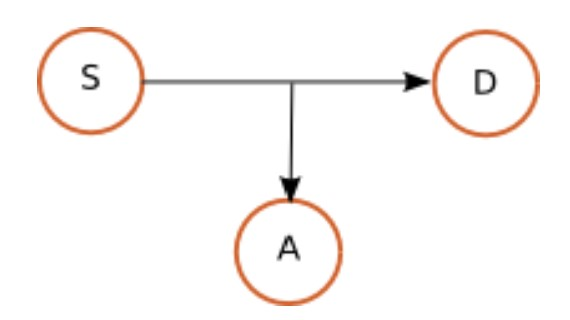
\includegraphics[scale = 0.7]{img/sec2.jpg}
    \label{sec2}
    \caption{The attacker intercepts information}
\end{figure}

Notice that in this case the attacker is \textbf{not modifying the information}, so this attack breaks the \textbf{confidentiality} of the system, since the information is accessed by unauthorized users. Differently from interruptions, interceptions are \textbf{quite difficult to detect}, and some examples are represented by unauthorized copies of programs or files or the interception of data flowing in the network (e.g. a credit card number).

\subsubsection{Modification}
In this case the \textbf{attacker modifies information}. To modify information, the attacker first \textbf{intercepts} it:

\begin{figure}[h!]
    \centering
    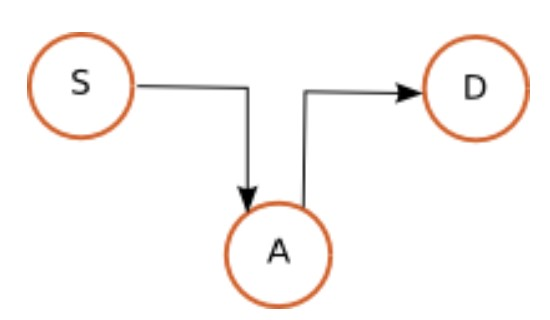
\includegraphics[scale = 0.7]{img/sec3.jpg}
    \label{sec3}
    \caption{The attacker modifies information}
\end{figure}

This attack breaks \textbf{integrity} and \textbf{confidentiality}, because the information is modified, thus accessed, by unauthorized users. Some examples involve unauthorized change of values (e.g. of a DB), of a program, or of data flowing in a network.

\subsubsection{Forging (or falsification)}
In this case the \textbf{attacker introduces new information}. This is usually related to \textbf{impersonation}, since the attacker lets the destination believe the information is coming from the honest source:

\begin{figure}[h!]
    \centering
    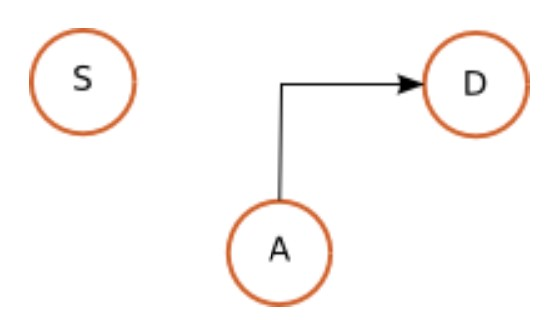
\includegraphics[scale = 0.7]{img/sec4.jpg}
    \label{sec4}
    \caption{The attacker forges new information}
\end{figure}

This attack breaks \textbf{authenticity} (since the attacker is not correctly identified), \textbf{accountability} (since it is not possible to trace the event to the attacker) and \textbf{integrity} (since we generate a message from nothing). Examples of forging involves the addition of new messages in the network, or the addition of a record in the DB.

In general, we distinguish \textbf{two types of attacks}, as shown in Picture \ref{sec8}.

\begin{figure}[h!]
    \centering
    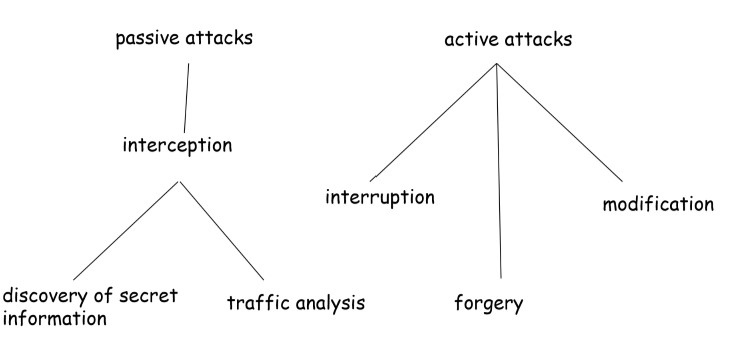
\includegraphics[scale = 1.2]{img/sec8.jpg}
    \label{sec8}
    \caption{Passive and active attacks}
\end{figure}

\subsubsection{Examples}
We give two simple examples of attacks to show how the general scenarios above apply.

\begin{enumerate}
    \item Suppose a bank B is using the following simple protocol to allow a bank transfer from user Alice (A):
    
    $$A \xrightarrow{} B: \text{sign}\_A(\text{“please pay Andy 1000 Euros”})$$
    
    ,where $\text{sign}\_A$ is some “signature” mechanism to ensure that the message really comes from Alice. We thus assume that the attacker cannot generate valid signed messages from Alice. However, it is always possible for the attacker to intercept the whole message and repeat it as many times as he wants, without modifying it. This attack, called \textbf{replay}, consists of an \textbf{interception} plus \textbf{forging} (in this case a very simple one as the message is just re-sent as is):

    \begin{figure}[h!]
        \centering
        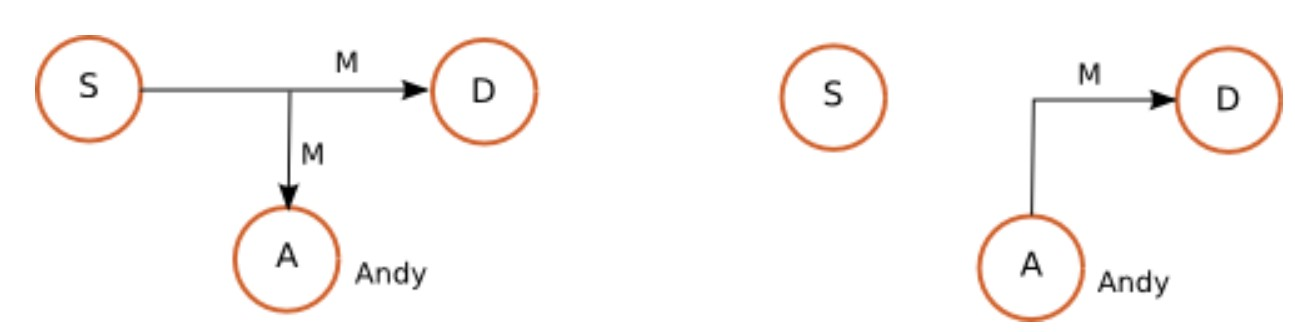
\includegraphics[scale = 0.7]{img/sec7.jpg}
        \label{sec7}
        \caption{The attacker Andy intercept the signed message and then replays it}
    \end{figure}

    In this way Andy gets the bank transfer as many times as he wants by just resending message M;

    \item A \textit{Trojan Horse} is a program that seems to behave as expected but incorporates malicious code (such as the Greek force hidden inside the mythological Trojan Horse as described in the Virgil’s Aeneid). These programs are usually obtained by modifying existing, honest programs. This is in fact an example of modification attack in which $S$ is the web site where the honest program $H$ can be downloaded and $D$ is the final user. The attacker downloads the honest program, modifies it and sets up a fake download site where $D$ will download the \textit{Trojan Horse} program.

    \begin{figure}[h!]
        \centering
        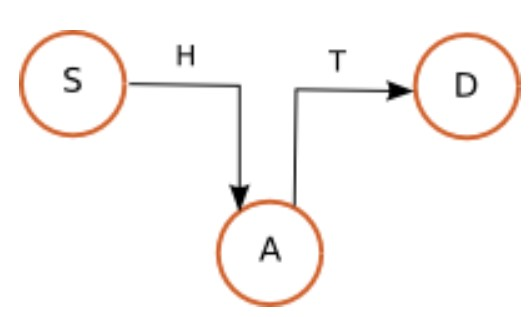
\includegraphics[scale = 0.7]{img/sec6.jpg}
        \label{sec6}
        \caption{The honest program $H$ is modified into a Trojan $T$}
    \end{figure}

    Such a program apparently works normally, however it changes, e.g., all the access rules of the users that is executing it. In this case is an attack to confidentiality and integrity.
\end{enumerate}



